\documentclass{ieeeaccess}
\usepackage{dsfont} %for \mathds command
%\usepackage{fullminipage}
\usepackage{epsfig}
\usepackage[cmex10]{amsmath}
\usepackage{graphicx}
\usepackage{pdfpages}
\usepackage{float}
\usepackage{amsfonts}
\usepackage{amsmath}
\usepackage{amssymb}
\usepackage{cite}
%\usepackage{floatrow}
\usepackage{bm}
\usepackage{mathrsfs}
\usepackage{subfig}
\usepackage{mathtools}
%\usepackage[ruled,vlined,linesnumbered]{algorithm2e}
\usepackage{arydshln}
\usepackage{inputenc}
\usepackage{algorithm}
\usepackage{algpseudocode}
%\usepackage{stfloats}
\usepackage{booktabs}
\newcommand*{\thead}[1]{\multicolumn{1}{c}{\bfseries #1}}
%\usepackage{algorithmic}
\usepackage{color}
\usepackage{amstext}
\usepackage{nomencl}
\usepackage{url}
\def\UrlBreaks{\do\/\do-}
\renewcommand{\UrlFont}{\small\tt}
\usepackage{multirow}
\usepackage{appendix}
\usepackage{verbatim}
\usepackage{longtable}
\usepackage{rotating}
\usepackage{fancyhdr}% fancyhdr related command; details in its documentation
%\graphicspath{{figures/}}
\DeclarePairedDelimiter{\abs}{\lvert}{\rvert}
\newcommand{\COMMENT}[1]{$\triangleright$  #1}
\usepackage{cite}
\usepackage{amsmath,amssymb,amsfonts}
\usepackage{algorithmic}
\usepackage{graphicx}
\usepackage{textcomp}

% Added by Vj
\usepackage{algpseudocode}


\def\BibTeX{{\rm B\kern-.05em{\sc i\kern-.025em b}\kern-.08em
    T\kern-.1667em\lower.7ex\hbox{E}\kern-.125emX}}
\begin{document}
\history{Date of publication xxxx 00, 0000, date of current version xxxx 00, 0000.}
\doi{10.1109/ACCESS.2017.DOI}

\title{Dynamic Delivery of Digital Video Using Multi-objective Optimization}
\author{
\uppercase{Gangadharan Esakki}\authorrefmark{1},      \IEEEmembership{?Student Member, IEEE}, \\
\uppercase{Venkatesh Jatla-Testing-Git}\authorrefmark{1},          \IEEEmembership{?Student Member, IEEE},  \\
\uppercase{Andreas S. Panayides}\authorrefmark{1,2,3} \IEEEmembership{Senior Member, IEEE}, and \\
\uppercase{Marios S. Pattichis}\authorrefmark{1},     \IEEEmembership{Senior Member, IEEE}}
\address[1]{
Image and Video Processing and Communications Lab 
Department of Electrical and Computer Engineering 
The University of New Mexico
Albuquerque, New Mexico, NM 87131 USA
(e-mails: , pattichi)}
\address[2]{SiGiNT Solutions Ltd, 2311 Nicosia, Cyprus (e-mail: a.panayides@sigintsolutions.com)}
\address[3]{Department of Computer Science, University of Cyprus, 1678 Nicosia, Cyprus (e-mail: panayides@cs.ucy.ac.cy)}
\tfootnote{
???? This paragraph of the first footnote will contain support 
information, including sponsor and financial support acknowledgment. For 
example, ``This work was supported in part by the U.S. Department of 
Commerce under Grant BS123456.''}

\markboth
{Author \headeretal: Preparation of Papers for IEEE TRANSACTIONS and JOURNALS}
{Author \headeretal: Preparation of Papers for IEEE TRANSACTIONS and JOURNALS}

\corresp{Corresponding author: First A. Author (e-mail: author@ boulder.nist.gov).}

\begin{abstract}
???
\end{abstract}

\begin{keywords}
???
e-mail to keywords@ieee.org or visit \underline
{http://www.ieee.org/organizations/pubs/ani\_prod/keywrd98.txt}
\end{keywords}

\titlepgskip=-15pt

\maketitle

\section{Introduction}
\label{sec:introduction}
\PARstart{T}{his} document is a template for \LaTeX. 
You can also explore using the Overleaf editor at 
\underline
{https://www.overleaf.com/blog/278-how-to-use-overleaf-}\break\underline{with-ieee-collabratec-your-quick-guide-to-getting-started}\break\underline{\#.xsVp6tpPkrKM9}

Start with the Problem Description and state clearly the motivation, approach, and benefits/ added value of your proposed solution. 
At the end of the Section and before Section 2 you need to provide a paragraph detailing how the paper is organized and what will follow in the next sections. A couple of sentences per section.


\section{Video Codecs for Adaptive Video Delivery}
Start with a brief paragraph introduction of what this Section covers. 

\subsection{Timeline}
Briefly mention when each codec was released and by which entity. Especially for the codecs that are investigated here include the official reference.

\subsection{Overview}
\subsubsection{VP9}
\subsubsection{H.265/HEVC}
\subsubsection{AV1}
\subsubsection{VVC}
Blah blah

\subsection{Adaptive Video Streaming}
blah blah

\section{Subjective and Objective Video Codecs Performance Evaluation}
This is Chapter 7 of Ganga's PhD, provide a brief description.
\subsection{Video Datasets}
This is 7.2.2 - Video Content Description
\subsection{Experimental Setup}
7.2.3 Video Codec Configuration Setup
\subsection{Video Quality Assessment (VQA)}
\subsubsection{Objective VQA}
\paragraph{PSNR611}
\paragraph{VMAF}
\paragraph{BD-RATE}
\subsubsection{Subjective VQA}
Describe the procedure
\paragraph{Correlation Metrics}
SROOCC and POCC

\subsection{Results}
Copy the appropriate Graph and Tables per Subsection
\subsubsection{HEVC Dataset}
\paragraph{240p}
blah
\paragraph{480p}
blah
\paragraph{720p}
blah
\paragraph{1080p}
blah
\paragraph{1600p}
blah
\paragraph{2500p}
blah
\subsubsection{UT LIVE Dataset}
\subsubsection{Tampere Dataset}
\subsubsection{Objective VQA Summary Results}
blah
\subsubsection{Subjective Evaluation Results}
blah

\section{Adaptive Video Delivery using Multi-objective Optimization}
\label{sec:adaptive video delivery}

\subsection{DRASTIC Multi-objective Optimization Framework}

\subsection{Adaptive Video Encoding}

\subsubsection{Segment Based Encoding}

\subsubsection{Experimental Setup}

\subsubsection{Forward Prediction Models Generation}
{Head and shoulders shots of authors that appear at the end of our papers. }

\subsubsection{Inverse Prediction Models for Real-time Video Encoding}
{Data charts which are typically black and white, but sometimes include 
color.}

\subsection{Results}

\subsubsection{Forward Prediction Models per Investigated Video Codec}

\paragraph{VP9}
\paragraph{H.265/HEVC}
\paragraph{AV1}
\paragraph{VVC}

\subsubsection{Adaptive Video Encoding per Investigated Video Codec and DRASTIC mode}

\paragraph{VP9}
\subparagraph{Maximum Video Quality}
\\
\subparagraph{Minimum Video Bitrate}
\paragraph{H.265/HEVC}
\subparagraph{Maximum Video Quality}
\\
\subparagraph{Minimum Video Bitrate}
\paragraph{AV1}
\subparagraph{Maximum Video Quality}
\\
\subparagraph{Minimum Video Bitrate}
\paragraph{VVC}
\subparagraph{Maximum Video Quality}
\\
\subparagraph{Minimum Video Bitrate}

\section{Discussion}

\subsection{Video Codecs Performance Evaluation}

\subsection{Adaptive Video Encoding}

\section{Concluding Remarks}
\appendices
Appendixes, if needed, appear before the acknowledgment.

\section*{Acknowledgment}
The preferred spelling of the word ``acknowledgment'' in American English is 
without an ``e'' after the ``g.'' Use the singular heading even if you have 
many acknowledgments. Avoid expressions such as ``One of us (S.B.A.) would 
like to thank $\ldots$ .'' Instead, write ``F. A. Author thanks $\ldots$ .'' In most 
cases, sponsor and financial support acknowledgments are placed in the 
unnumbered footnote on the first page, not here.

\begin{IEEEbiography}[{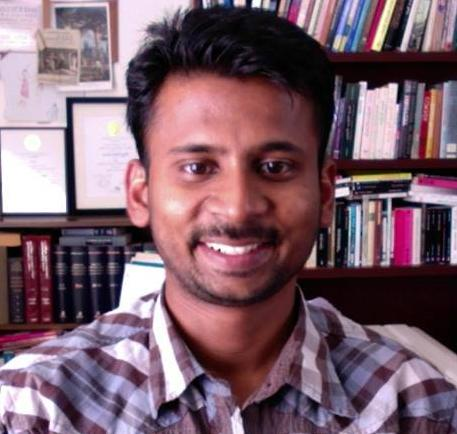
\includegraphics[width=1in,height=1.25in,clip,keepaspectratio]{pictures/authors/ganga.jpg}}]{Gangadharan Esakki} (M'76--SM'81--F'87) ???
\end{IEEEbiography}

\begin{IEEEbiography}[{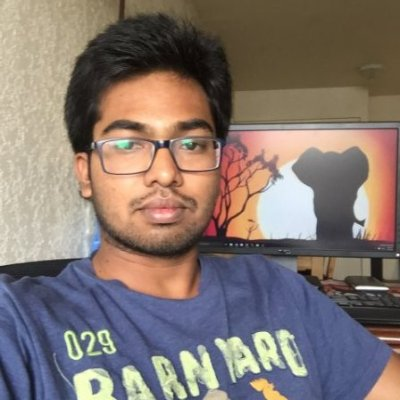
\includegraphics[width=1in,height=1.25in,clip,keepaspectratio]{pictures/authors/vj.jpg}}]{Venkatesh Jatla} ???
\end{IEEEbiography}

\begin{IEEEbiography}[{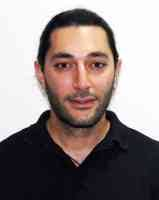
\includegraphics[width=1in,height=1.25in,clip,keepaspectratio]{pictures/authors/andreas.jpg}}]{Andreas S. Panayides} (M'87) 
???
\end{IEEEbiography}

\begin{IEEEbiography}[{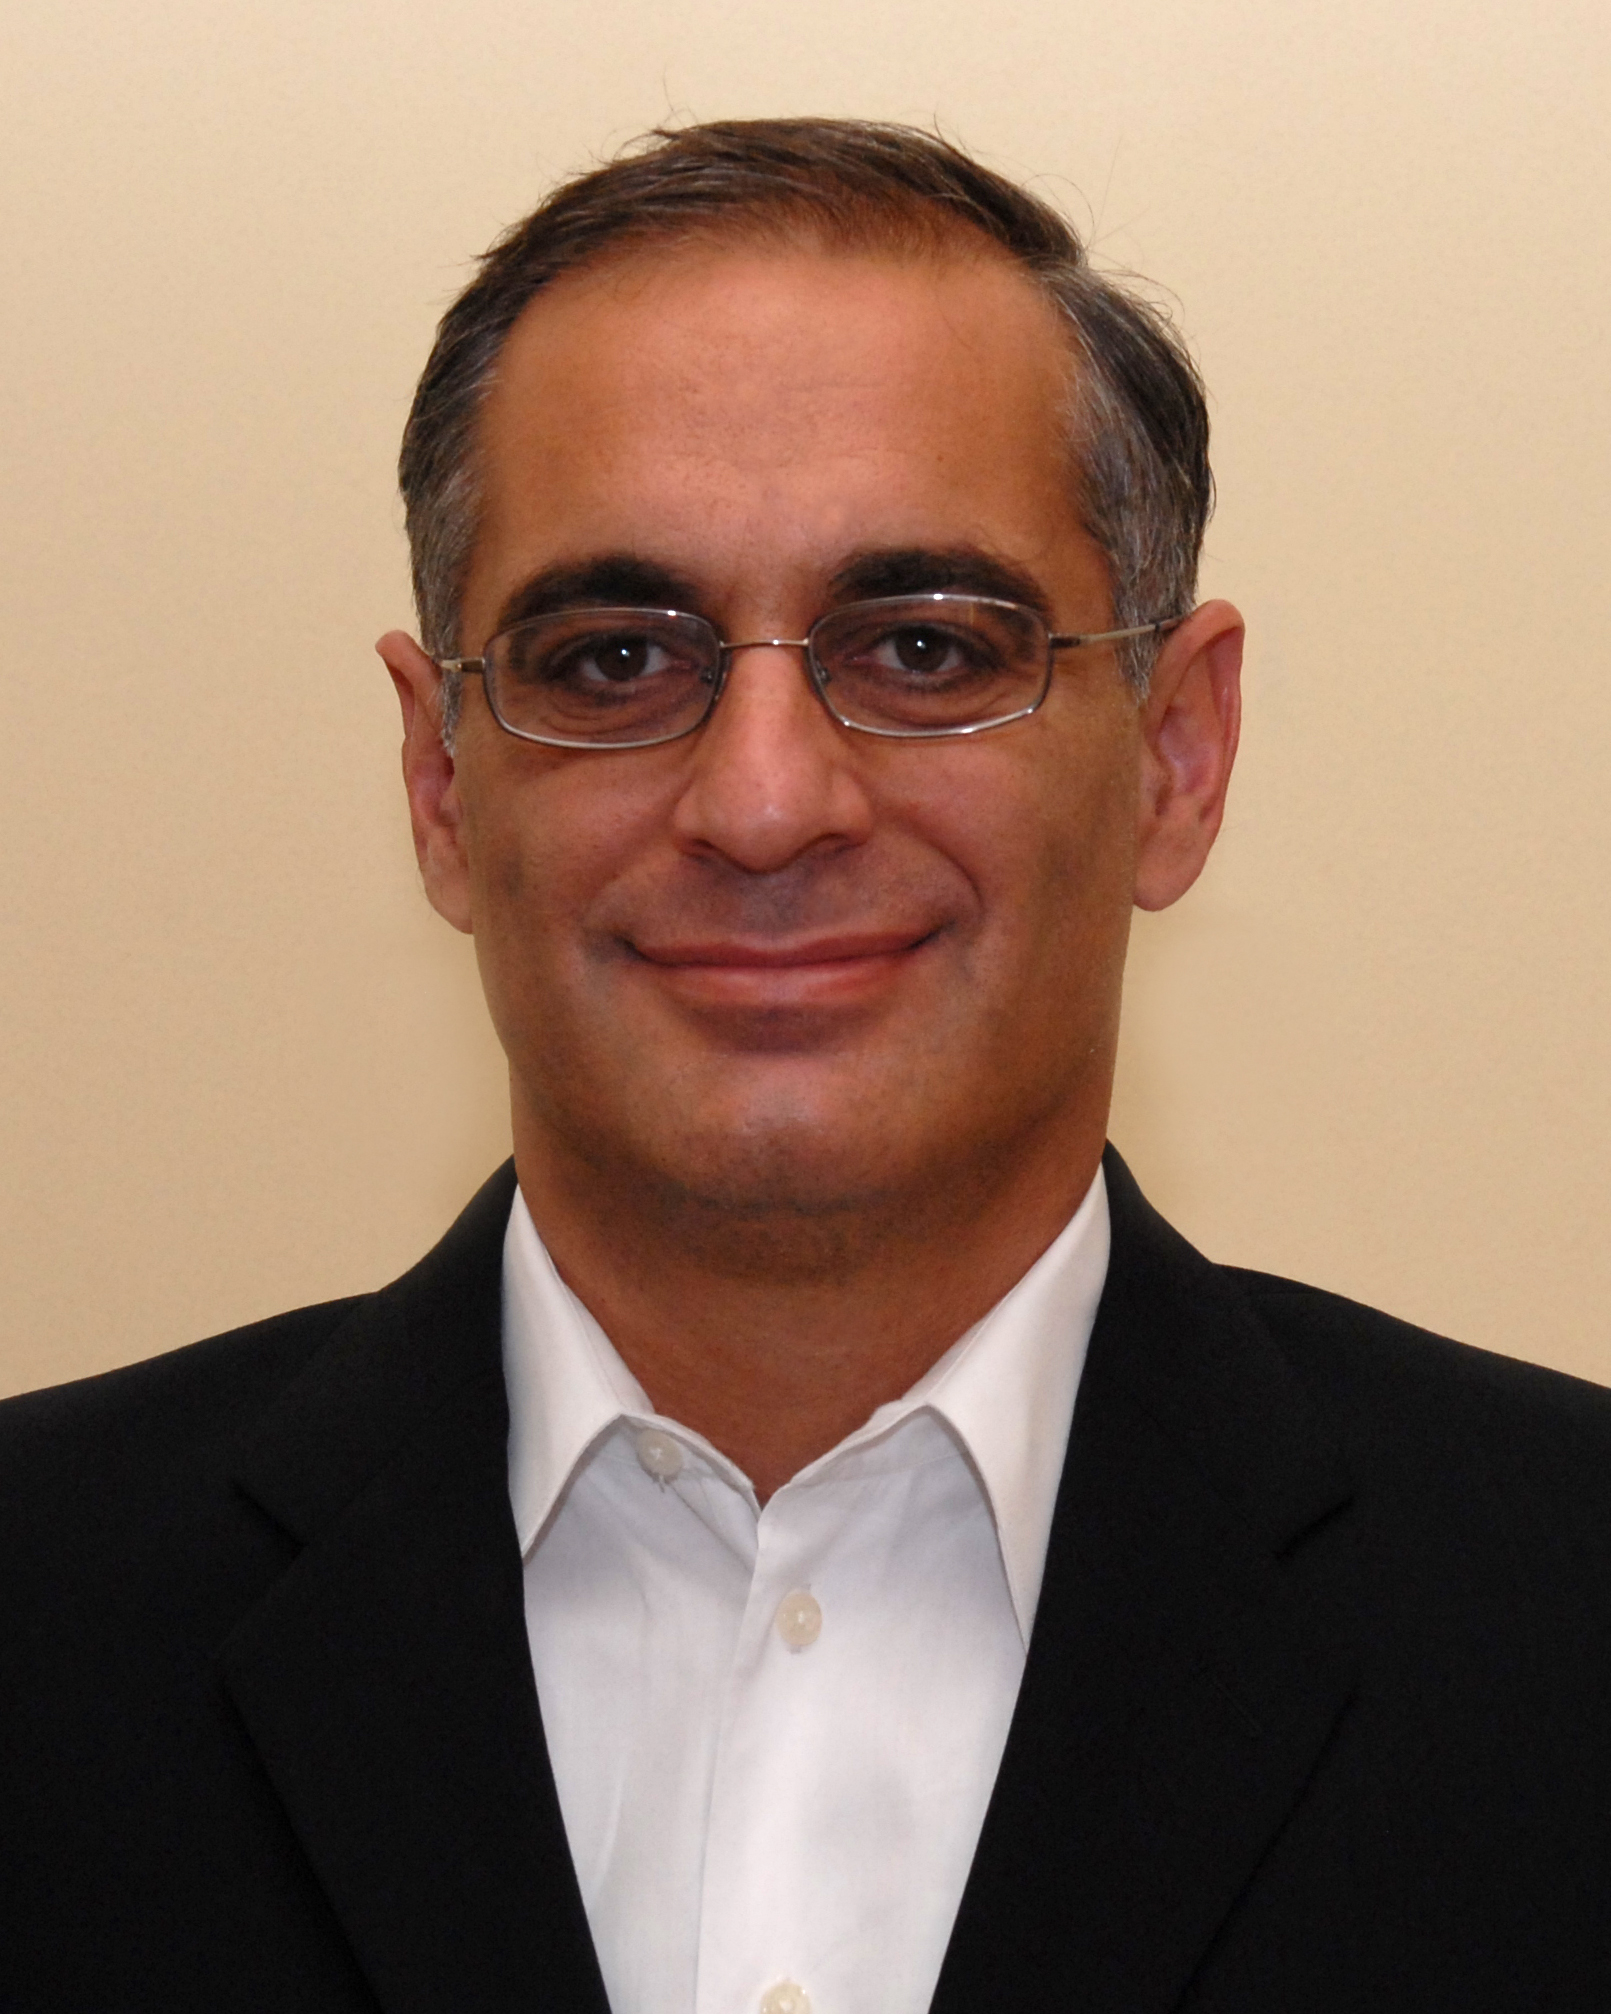
\includegraphics[width=1in,height=1.25in,clip,keepaspectratio]{pictures/authors/Pattichis.jpg}}]{Marios S. Pattichis} (M'87) 
???
\end{IEEEbiography}

\EOD
\end{document}
